\section*{Research Methodology}
This study adopts a structured, phased methodology to formulate, analyze, and validate optimization models for three-layer Collaborative Edge Inference (CEI) \cite{qu2024elastic,mcenroe2022survey}. The phased design progresses from preliminary trade-off analysis, through formal problem formulation and solution, to online adaptation and empirical validation via network--robotics co-simulation \cite{hu2025splitreview,blanquer2024resilient,duan2022combined,li2024fsl,jung2024edgeai,adoni2024intelligent,kabashkin2024resilience,clerigues2024mission,wang2024ress}.

\subsection*{Preliminary Analysis}

To expose the fundamental structure of the problem, we conduct a simplified analysis of latency--energy trade-offs under different partitioning regimes. We consider a setting in which a DNN is partitioned into multiple segments and executed across a team of UAVs. Configurations with fewer partitions concentrate computation on fewer nodes (higher per-node latency, lower communication overhead), while finer partitioning distributes load but incurs more frequent tensor exchanges. Partitioning decisions therefore jointly determine both computation load distribution and communication requirements.

\begin{figure}[H]
  \centering
  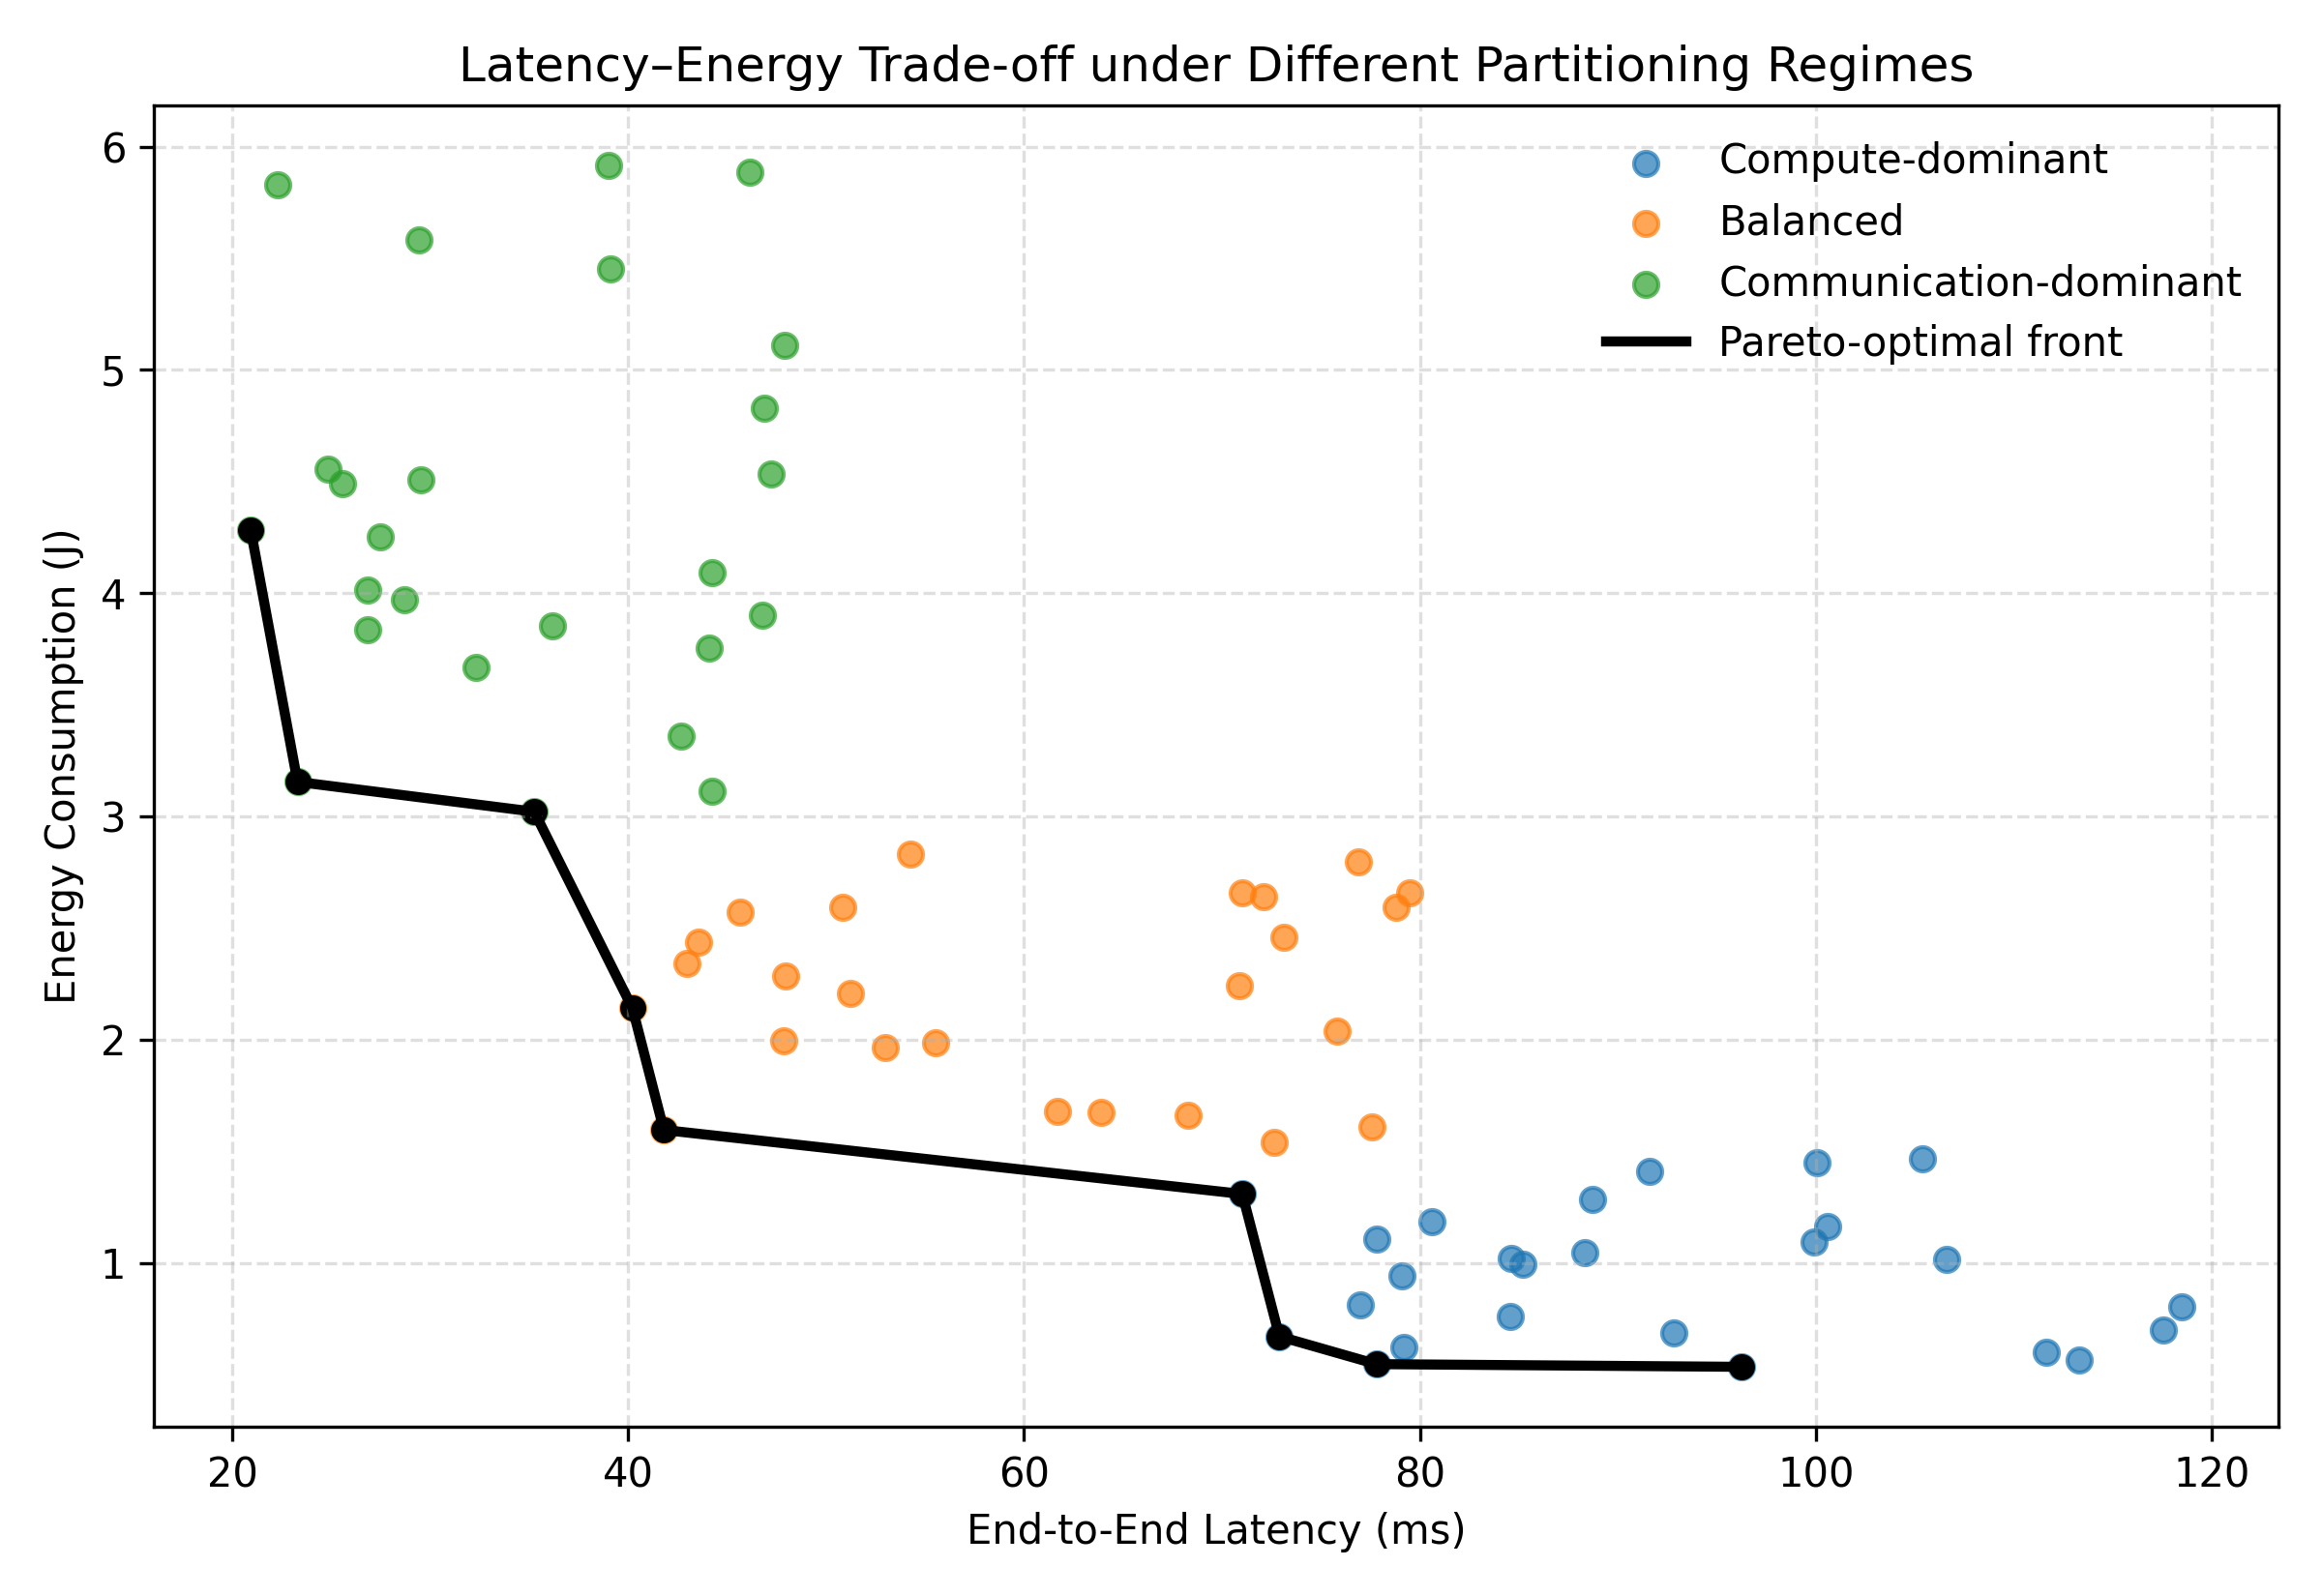
\includegraphics[width=0.85\linewidth]{image/pareto_preliminary_clean.png}
  \caption{Illustrative latency--energy trade-off under different partitioning regimes. Each point corresponds to a specific partitioning--assignment configuration; clusters represent computation-dominant, communication-dominant, and balanced regimes. The Pareto front shows the set of non-dominated solutions.}
  \label{fig:pareto}
\end{figure}

Fig.~\ref{fig:pareto} shows the resulting operating points in latency--energy space, generated from a simplified simulation under homogeneous UAV capabilities and static links. Three distinct regimes are visible: computation-dominant configurations (lower energy, higher latency), communication-dominant configurations (lower latency, higher energy), and balanced configurations between the extremes. The Pareto front confirms that no single configuration simultaneously minimizes both objectives---any improvement in one dimension requires a trade-off in the other.

This trade-off structure cannot be resolved through independent optimization of computation or communication, confirming that a joint formulation is necessary. The simplified setting is intended solely to reveal this structural insight; more realistic conditions (heterogeneous UAVs, dynamic links) are addressed in the full formulation and evaluation.

\subsection*{Problem Formulation}
Collaborative inference is modeled as a sequential AI pipeline comprising ordered computational stages \cite{kang2017neurosurgeon,matsubara2022split}. The model is represented by a bounded-$K$ partition family, where $K$ denotes the number of partitions and is restricted to a small value to balance analytical tractability against communication overhead. Each partition is assigned to exactly one UAV through binary decision variables, subject to per-node computation and energy constraints and execution-order preservation.

When two consecutive partitions are mapped to different UAVs, an intermediate tensor is transmitted along the FANET path between the corresponding nodes. End-to-end latency is modeled as the sum of partition-level computation delays and inter-partition transmission delays; total energy combines onboard computation energy and RF transmission energy. Crucially, partition boundaries determine intermediate tensor sizes, creating a feedback loop between computation placement and communication cost.

We formulate the problem as
\[
\min_{x \in \mathcal{X}} \; L(x) + \lambda E(x),
\]

where
\begin{itemize}
    \item $L(x)$ denotes end-to-end inference latency,
    \item $E(x)$ denotes total system energy consumption (computation and RF communication),
    \item $\lambda \geq 0$ is a trade-off parameter balancing latency and energy.
\end{itemize}

The decision variable $x$ comprises model partitioning decisions and UAV assignment decisions. The feasible set $\mathcal{X}$ is defined by SWaP constraints (compute, memory, energy), communication constraints over the FANET, and sequential execution constraints induced by model partitioning.

\paragraph{Computational Complexity.}
The joint problem is combinatorial, with complexity growing exponentially in the number of candidate partition points and UAV nodes. Exact solutions are therefore intractable for real-time deployment in dynamic environments, motivating the bounded-$K$ restriction and the investigation of tractable approximation strategies.

\subsection*{1. Theoretical Foundation of Joint Partitioning and Assignment}
The first phase addresses RQ1 by formulating the combinatorial optimization problem under SWaP constraints \cite{qu2024elastic,hu2025splitreview,duan2022combined,li2024fsl,kang2017neurosurgeon,hu2019dads,zhao2025joint}. The formulation defines decision variables for bounded-$K$ partition selection and binary UAV assignment, then minimizes the coupled latency--energy objective.

The key challenge is that partitioning and assignment are inseparable: partition boundaries determine tensor sizes that affect communication cost, which in turn constrains feasible assignments. The scientific contribution of this phase is a structured analysis of this interdependence and of the role of $K$ in problem complexity, including identification of tractable substructures and approximation opportunities \cite{hu2025splitreview,mcenroe2022survey}.

\begin{figure}[H]
  \centering
  \resizebox{0.85\textwidth}{!}{\centering
\resizebox{\linewidth}{!}{%
  \begin{tikzpicture}[
      font=\sffamily,
      >=Stealth,
      model_block/.style={rectangle, draw=blue!80!black, thick, top color=white, bottom color=blue!10, minimum width=3.8cm, minimum height=1.2cm, rounded corners=2mm, drop shadow, align=center},
      uav_node/.style={rectangle, draw=orange!80!black, thick, top color=white, bottom color=orange!10, minimum width=4cm, minimum height=1.5cm, rounded corners=2mm, drop shadow, align=center},
      data_arrow/.style={->, thick, blue!70!black},
      mapping_arrow/.style={->, thick, gray, dotted},
      wireless_arrow/.style={->, thick, dashed, orange!90!black, decorate, decoration={snake, amplitude=.4mm, segment length=3mm, post length=2mm}},
      group_box/.style={rectangle, draw=black!30, dashed, thick, inner sep=12pt, rounded corners=3mm}
    ]

    % ================= LEFT: LOGICAL AI MODEL =================
    \node (input) {\textbf{Input Data (Images/Video)}};
    \node[model_block, below=0.6cm of input] (l1) {\textbf{Partition $p_1$} \\ \scriptsize Early Layers};
    \node[model_block, below=1.2cm of l1] (l2) {\textbf{Partition $p_i$} \\ \scriptsize Intermediate Layers};
    \node[model_block, below=1.2cm of l2] (l3) {\textbf{Partition $p_K$} \\ \scriptsize Late/Output Layers};
    \node[below=0.8cm of l3] (output) {\textbf{Inference Result}};

    \draw[data_arrow] (input) -- (l1);
    \draw[data_arrow] (l1) -- node[right, font=\scriptsize\bfseries, blue!80!black] {Cut-point $c_i$} (l2);
    \draw[data_arrow] (l2) -- node[right, font=\scriptsize\bfseries, blue!80!black] {Cut-point $c_{i+1}$} (l3);
    \draw[data_arrow] (l3) -- (output);

    \begin{scope}[on background layer]
      \node[group_box, fill=blue!2, fit=(input) (l1) (l2) (l3) (output)] (model_bg) {};
      \node[above=5pt of model_bg.north, font=\bfseries\large, blue!80!black] {Logical AI Model (Bounded-$K$ Partition)};
    \end{scope}

    % ================= RIGHT: PHYSICAL UAV SWARM =================
    \node[uav_node, right=4.5cm of l1] (u1) {\textbf{UAV 1} (Cluster Head)\\ \vspace{1mm} \scriptsize \textcolor{black!70}{CPU: 80\% |} \textbf{\textcolor{green!60!black}{Battery: High}}};
    \node[uav_node, right=4.5cm of l2] (u2) {\textbf{UAV 2} (Worker Node)\\ \vspace{1mm} \scriptsize \textcolor{black!70}{GPU: 95\% |} \textbf{\textcolor{orange!90!black}{Battery: Medium}}};
    \node[uav_node, right=4.5cm of l3] (u3) {\textbf{UAV 3} (Worker Node)\\ \vspace{1mm} \scriptsize \textcolor{black!70}{CPU: 40\% |} \textbf{\textcolor{red!80!black}{Battery: Low}}};

    \begin{scope}[on background layer]
      \node[group_box, fill=orange!3, fit=(u1) (u2) (u3)] (swarm_bg) {};
      \node[above=5pt of swarm_bg.north, font=\bfseries\large, orange!80!black] {Physical UAV Swarm (FANET)};
    \end{scope}

    % ================= MAPPING AND WIRELESS =================
    % Mapping arrows: tăng khoảng cách nhãn
    \draw[mapping_arrow] (l1.east) to[out=0, in=180] node[pos=0.6, above, sloped, font=\scriptsize\itshape, black!70] {Dynamic Allocation} (u1.west);
    \draw[mapping_arrow] (l2.east) to[out=0, in=180] node[pos=0.6, above, sloped, font=\scriptsize\itshape, black!70] {Dynamic Allocation} (u2.west);
    \draw[mapping_arrow] (l3.east) to[out=0, in=180] node[pos=0.6, above, sloped, font=\scriptsize\itshape, black!70] {Dynamic Allocation} (u3.west);

    % Wireless arrows: tăng khoảng cách nhãn "Transmit Tensor" và làm thoáng hơn
    \draw[wireless_arrow] (u1.south) -- node[pos=0.50, right, font=\scriptsize\bfseries, orange!90!black] {Transmit Tensor $T_1$} (u2.north);
    \draw[wireless_arrow] (u2.south) -- node[pos=0.50, right, font=\scriptsize\bfseries, orange!90!black] {Transmit Tensor $T_2$} (u3.north);

  \end{tikzpicture}%
}
}
  \caption{Collaborative edge inference with a simplified three-partition example under a bounded-$K$ model, illustrating how partition boundaries induce intermediate tensor transmissions between UAVs.}
  \label{fig:architecture}
\end{figure}

\subsection*{2. Communication-Cost Modeling under Coupled Optimization}
Building on the joint model, the second phase completes RQ1 by formalizing communication cost over volatile FANETs \cite{lansky2023firefly,hosseinzadeh2024local,blanquer2024resilient,rahmani2021fanet,clerigues2024mission}. The goal is to characterize communication delay and RF energy as functions of tensor size, available bandwidth, and link variation, then embed these terms in the global objective.

The key challenge is that communication cost is not an external parameter but a quantity induced by partition decisions---it changes whenever the optimization variables change. The scientific contribution is a communication-aware cost model that preserves this dependency and supports latency--energy trade-off analysis across different mobility regimes \cite{lansky2023firefly,hosseinzadeh2024local,qu2024elastic,wang2024ress,lucchesi2024dynamic,shao2020bottlenet,shao2022task,li2023device}.

\begin{figure}[H]
  \centering
  \resizebox{0.85\textwidth}{!}{\centering
\begin{tikzpicture}[
    font=\sffamily,
    >=Stealth,
    % Styles cho các khối xử lý
    feature_block/.style={
      rectangle, draw=blue!70, thick, fill=blue!5,
      minimum width=3.2cm, minimum height=1.1cm,
      rounded corners=2mm, align=center,
      font=\small
    },
    compress_block/.style={
      rectangle, draw=red!70, thick, fill=red!5,
      minimum width=3.2cm, minimum height=1.1cm,
      rounded corners=2mm, align=center,
      font=\small
    },
    uav_group/.style={
      rectangle, draw=black!40, dashed, thick,
      rounded corners=3mm, inner sep=12pt,
      fill=gray!3
    },
    % Arrow styles
    flow_arrow/.style={->, thick, blue!60},
    wireless_arrow/.style={<->, thick, dashed, orange!80,
    decorate, decoration={snake, amplitude=0.3mm, segment length=3mm, post length=1mm}},
    label/.style={font=\scriptsize\itshape},
    % Khoảng cách giữa các node
    node distance=1.2cm and 3cm
  ]

  % ===== UAV 1 (Sender) – bên trái =====
  \node[align=center] (sensor) {\textbf{Sensor Data} \\ \scriptsize Images/Video};

  \node[feature_block, below=of sensor] (front) {Front AI Layers \\ \scriptsize Feature Extraction};

  \node[compress_block, below=of front] (compress) {Tensor Compression \\ \scriptsize Quantization};

  % Mũi tên trong UAV 1
  \draw[flow_arrow] (sensor) -- (front);
  \draw[flow_arrow] (front) -- node[right, label] {Intermediate Tensor $T$} (compress);

  % Nhóm UAV 1
  \begin{scope}[on background layer]
    \node[uav_group, fit=(sensor) (front) (compress)] (uav1) {};
    \node[above=4pt of uav1.north, font=\small\bfseries] {UAV Node 1 (Sender / Edge)};
  \end{scope}

  % ===== UAV 2 (Receiver) – bên phải, đặt ngang hàng với UAV1 =====
  % Dùng positioning: right=of uav1.east, nhưng để căn chỉnh theo tâm của UAV1, ta đặt node (decompress) ở vị trí phù hợp
  \node[compress_block, right=4.5cm of compress] (decompress) {Tensor Decompression \\ \scriptsize Reconstruction};

  \node[feature_block, below=of decompress] (tail) {Tail AI Layers \\ \scriptsize Classifier};

  \node (result) [below=of tail] {\textbf{Inference Result}};

  % Mũi tên trong UAV 2
  \draw[flow_arrow] (decompress) -- (tail);
  \draw[flow_arrow] (tail) -- (result);

  % Nhóm UAV 2
  \begin{scope}[on background layer]
    \node[uav_group, fit=(decompress) (tail) (result)] (uav2) {};
    \node[above=4pt of uav2.north, font=\small\bfseries] {UAV Node 2 (Receiver / Cluster Head)};
  \end{scope}

  % ===== Kết nối không dây =====
  \draw[wireless_arrow] (compress.east) --
  node[above, font=\small\bfseries, orange!80] {Compressed $T_c$}
  node[below, label, pos=0.5] {Energy-Efficient FANET}
  (decompress.west);

  % Điểm cắt (cut point)
  \node[font=\tiny\bfseries, text=red!70, above right=0pt and -2pt of compress.north east] {Cut Point};

\end{tikzpicture}
}
  \caption{Data flow and energy-aware communication protocol for CEI. The intermediate tensor ($T$) is compressed ($T_c$) before transmission to reduce bandwidth overhead and RF energy cost.}
  \label{fig:workflow}
\end{figure}

\subsection*{3. Online Re-optimization under Mobility and Failures}
The third phase addresses RQ2 as an online optimization problem \cite{pan2025selfhealing,jamshidi2025resilient,blanquer2024resilient,seid2021multiagent,gao2025pmdp}. This phase is necessary because the joint optimum from Phases~1--2 is state-dependent: topology changes, mobility, residual energy depletion, and node/link failures reshape both the objective value and the feasible set over time. A static solution therefore degrades as conditions evolve.

The adaptation framework is derived from the structural properties of the joint problem rather than introduced as an independent add-on. The phase studies how the coupled solution should be updated online in response to observed system state, and evaluates candidate approaches (control-theoretic and learning-based methods) under a unified structural framework.

\begin{figure}[H]
  \centering
  \resizebox{1\textwidth}{!}{\centering
\resizebox{1\textwidth}{!}{%
  \begin{tikzpicture}[
      font=\sffamily,
      >=Stealth,
      node distance=1.5cm and 2.5cm,
      % Styles
      ctrl_block/.style={
        rectangle, draw=purple!80!black, thick,
        top color=white, bottom color=purple!10,
        minimum width=6cm, minimum height=1.2cm,
        rounded corners=2mm, drop shadow, align=center,
        font=\small
      },
      uav_normal/.style={
        rectangle, draw=orange!80!black, thick,
        top color=white, bottom color=orange!10,
        minimum width=3.5cm, minimum height=1.2cm,
        rounded corners=2mm, drop shadow, align=center,
        font=\small
      },
      uav_failed/.style={
        rectangle, draw=red!70, thick, dashed,
        fill=gray!10, text=gray!60,
        minimum width=3.5cm, minimum height=1.2cm,
        rounded corners=2mm, align=center,
        font=\small
      },
      uav_backup/.style={
        rectangle, draw=green!60!black, thick,
        top color=white, bottom color=green!10,
        minimum width=3.5cm, minimum height=1.2cm,
        rounded corners=2mm, drop shadow, align=center,
        font=\small
      },
      cross_mark/.style={cross out, draw=red, thick, minimum size=1.3cm},
      % Arrows
      data_flow/.style={->, thick, dashed, orange!80},
      failed_link/.style={->, thick, dashed, red!50},
      ctrl_arrow/.style={->, thick, dashed, purple!70},
      alert_arrow/.style={->, thick, dotted, red!70},
    ]

    % Hàng trên: UAV 2 (failed)
    \node[uav_failed] (u2) {UAV 2 \\ \scriptsize (Offline)};

    % Hàng thứ hai: UAV 1 và UAV 3, thấp hơn và lệch sang hai bên
    \node[uav_normal, below=1cm of u2, xshift=-7.5cm] (u1) {UAV 1 \\ \scriptsize Partition 1};
    \node[uav_normal, below=1cm of u2, xshift=7.5cm] (u3) {UAV 3 \\ \scriptsize Partition 3};

    % Control plane: thẳng hàng dọc dưới u2
    \node[ctrl_block, below=2cm of u2] (cp) {Intelligent Control Plane \\ \scriptsize Telemetry Monitoring \& Dynamic Orchestration};

    % Backup UAV: thẳng hàng dọc dưới cp
    \node[uav_backup, below=1.5cm of cp] (u4) {UAV 4 (Backup) \\ \scriptsize \textbf{Reallocated:} Partition 2};

    % Dấu chéo trên UAV hỏng
    \node[cross_mark] at (u2.center) {};

    % Các đường "Link Down" nằm phía trên UAV 1 và 3
    \draw[failed_link] (u1.north) |- node[pos=0.6, above, font=\tiny\itshape, red!60] {(1) Link Down} (u2.west);
    \draw[failed_link] (u2.east) -| node[pos=0.4, above, font=\tiny\itshape, red!60] {(1) Link Down} (u3.north);

    % Đường reroute dữ liệu
    \draw[data_flow] (u1.south) |- node[pos=0.6, above, font=\tiny\bfseries, orange!80] {(4) Reroute $T_1$} (u4.west);
    \draw[data_flow] (u4.east) -| node[pos=0.4, above, font=\tiny\bfseries, orange!80] {(4) Reroute $T_2$} (u3.south);

    % Phản hồi từ UAV hỏng lên control plane
    \draw[alert_arrow] (u2.south) -- node[midway, font=\tiny\bfseries, red!70, fill=white] {(2) Failure Alert} (cp.north);

    % Tín hiệu điều khiển
    \draw[ctrl_arrow] (cp.north west) to[out=180, in=30, looseness=1.2] node[right, font=\tiny, purple!70] {(3) Update Routing} (u1.east);
    \draw[ctrl_arrow] (cp.north east) to[out=0,in=150, looseness=1.2] node[left, font=\tiny, purple!70] {(3) Update Source} (u3.west);
    \draw[ctrl_arrow] (cp.south) -- node[right, font=\tiny, purple!70] {(3) Deploy Partition 2} (u4.north);

    % Chú thích
    % \node[text=orange!80, below=0.2cm of u4.south, align=center] {New tensor paths};

  \end{tikzpicture}%
}
}
  \caption{Adaptive orchestration and fault tolerance by the intelligent control plane. When a UAV fails, the control plane reallocates missing partitions and reroutes tensors to maintain uninterrupted inference.}
  \label{fig:fault_tolerance}
\end{figure}

This phase is organized into three steps:
\begin{itemize}
  \item \textbf{Contextual Monitoring:} Define a telemetry state representation for continuous observation of link quality, packet loss, residual energy, CPU load, and graph execution status \cite{qu2024elastic,mcenroe2022survey}.
  \item \textbf{Online Decision Update:} Formulate a baseline re-optimization mechanism and extend it to multi-objective policies that update partitioning--assignment decisions as system conditions change \cite{pan2025selfhealing,jamshidi2025resilient}.
  \item \textbf{Dynamic Reconfiguration:} Apply reallocation and rerouting decisions---including repartitioning and tensor-path adaptation away from unstable nodes---to maintain uninterrupted inference \cite{pan2025selfhealing,blanquer2024resilient,hosseinzadeh2024local}.
\end{itemize}

Overall, this phase emphasizes decision quality over time rather than static deployment quality.

\paragraph{Risk Considerations.}
Several potential risks are acknowledged. First, scalability challenges may arise as the number of partitions increases; this is mitigated through bounded-$K$ design and investigation of tractable approximations. Second, discrepancies between simulation and real-world deployment may limit direct applicability; this is addressed by focusing on structural insights rather than system-specific tuning. Third, ethical considerations related to UAV applications are recognized, and the proposed framework is intended for civilian and research-oriented use cases.
